\newpage

\section{Ход работы}
%\label{sec:Chapter4} \index{Chapter4}

% Здесь немного описать как мы разбиваем выборку на подвыборки, вставить пару табличек
% с объектами, принадлежащими одному человеку.
% Объяснить для чего мы их разбиваем, сколько моделей берём 
% ...
% Возьмём самый простой метод -- логистическую регрессию.
Для того, чтобы рассмотреть каждый электрод по отдельности, необходимо разделить наши
исходные данные перед тем, как применять алгоритмы машинного обучения. Процесс разделения
исходных данных будет описан далее.

\subsection{Разделение данных}
\label{sec:chapter_5_1}

Разобьём наш исходный набор данных на "подвыборки", в каждой из которых будет информация,
относящаяся только к одному участнику эксперимента. Всего принимал участие в эксперименте
101 человек, следовательно, и подвыборок будет 101 (по одной на каждого человека). 
На рис. \ref{fig_5} показан пример одной из подвыборок.

\begin{figure}[H]
    \centering
    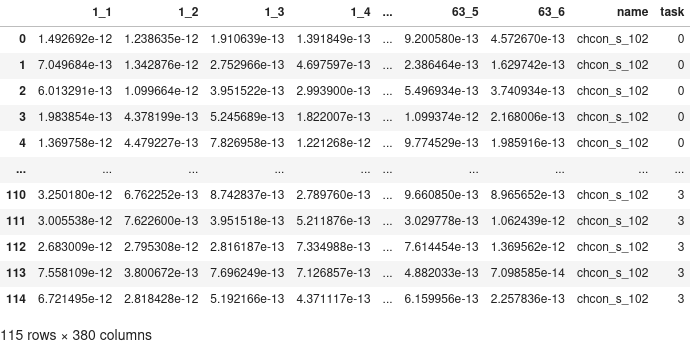
\includegraphics[width=\linewidth]{images/5.png}
    \caption{Пример набора данных для одного человека}
    \label{fig_5}
\end{figure}

Затем необходимо разделить полученные выборки так, чтобы в них содержалась информация
только об одном электроде. Каждый электрод характеризуется шестью частотными диапазонами
ЭЭГ (см. главу \ref{sec:chapter_3_2}). То есть в получившемся наборе данных (см. рис. \ref{fig_6}) для одного электрода будет шесть колонок
(не считая колонки "task" целевых переменных с типом сложности задачи).

\begin{figure}[H]
    \centering
    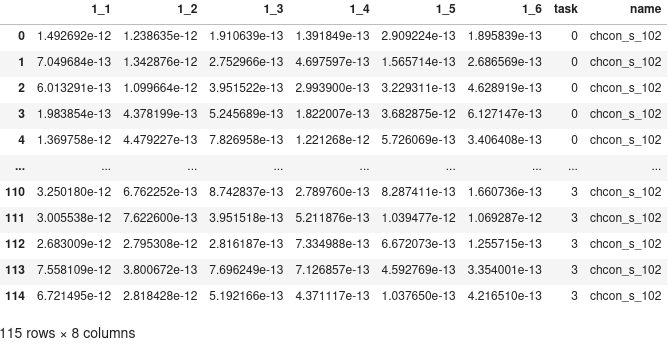
\includegraphics[width=\linewidth]{images/6.png}
    \caption{Пример получившегося набора данных для первого электрода (колонка $"name"$
    добавлена для наглядности).}
    \label{fig_6}
\end{figure}

Итого 63 получившихся набора данных для каждого человека. Всего таких наборов
$101\cdot 63=6363$. Количество строк в таком наборе от человека к человеку варьируется
от 80 до 120 (см. главу \ref{sec:chapter_3_3}).

Опишем формально получившийся набор данных. Получится выражение, аналогичное выражению
(\ref{eq:eq_1}), но изменится размерность $n$ и $l$:

\begin{equation}
    \label{eq:eq_2}
    \textbf{Обучающая выборка:\:} X^l=(x_i, y_i)_{i=1}^l,\quad x_i\in \mathbb{R}^n,\quad y_i\in\lbrace 0, 1, 2, 3\rbrace,
\end{equation}
где $\quad l\in[80, 120],\quad n=6$.\\[3 mm]
    
Итак, у нас есть обучающие выборки (по 63 на каждого участника эксперимента), каждой из которых соответствует пара объект-ответ. Объект
описывается шестью характеризующими электрод вещественными признаками — амплитудами
колебаний электромагнитной активности, а ответы — это числа от 0 до 3, соответствующие
типу решаемой задачи.

Учитывая небольшой размер данных (80-120 строк), с которыми нужно будет работать, возьмём
простой и широко используемый в задачах классификации метод --- логистическую регрессию.

\subsection{Логистическая регрессия}
\label{sec:chapter_5_2}

Логистическая регрессия применяется для предсказания вероятности возникновения
некоторого события по значениям множества признаков \cite{ML_lectures}. Для этого вводится
целевая переменная ${\displaystyle y}$.

\subsubsection{Описание}
1. \textit{Случай бинарной классификации}.\\[0.3 cm]
В этом случае зависимая переменная $y$, принимающая одно из двух значений---это
числа 0  и 1, и множество
независимых переменных (также называемых признаками, предикторами или регрессорами) ---
вещественных $x_{1},x_{2},\cdots,x_{n}$, на основе значений которых требуется вычислить
вероятность принятия того или иного значения целевой переменной. Как и в случае
линейной регрессии, для простоты записи вводится фиктивный признак $x_0 = 1$.\\
Делается предположение о том, что вероятность наступления события $y = 1$ равна:
\begin{equation*}
    {\mathbb {P}}\{y=1\mid x\}=f(z),
\end{equation*}
где $z=\theta ^{T}x=\theta _{0}+\theta _{1}x_{1}+\ldots +\theta_{n}x_{n}$, $x$ и $\theta$
--- векторы-столбцы значений независимых переменных $1$, $x_{1},\dots ,x_{n}$ и параметров
(коэффициентов регрессии) — вещественных чисел $\theta _{0},...,\theta _{n}$,
соответственно, а $f(z)$ --- так называемая логистическая функция (иногда также
называемая сигмоидой или логит-функцией): $f(z)={\frac {1}{1+e^{{-z}}}}$.

\begin{figure}[H]
    \centering
    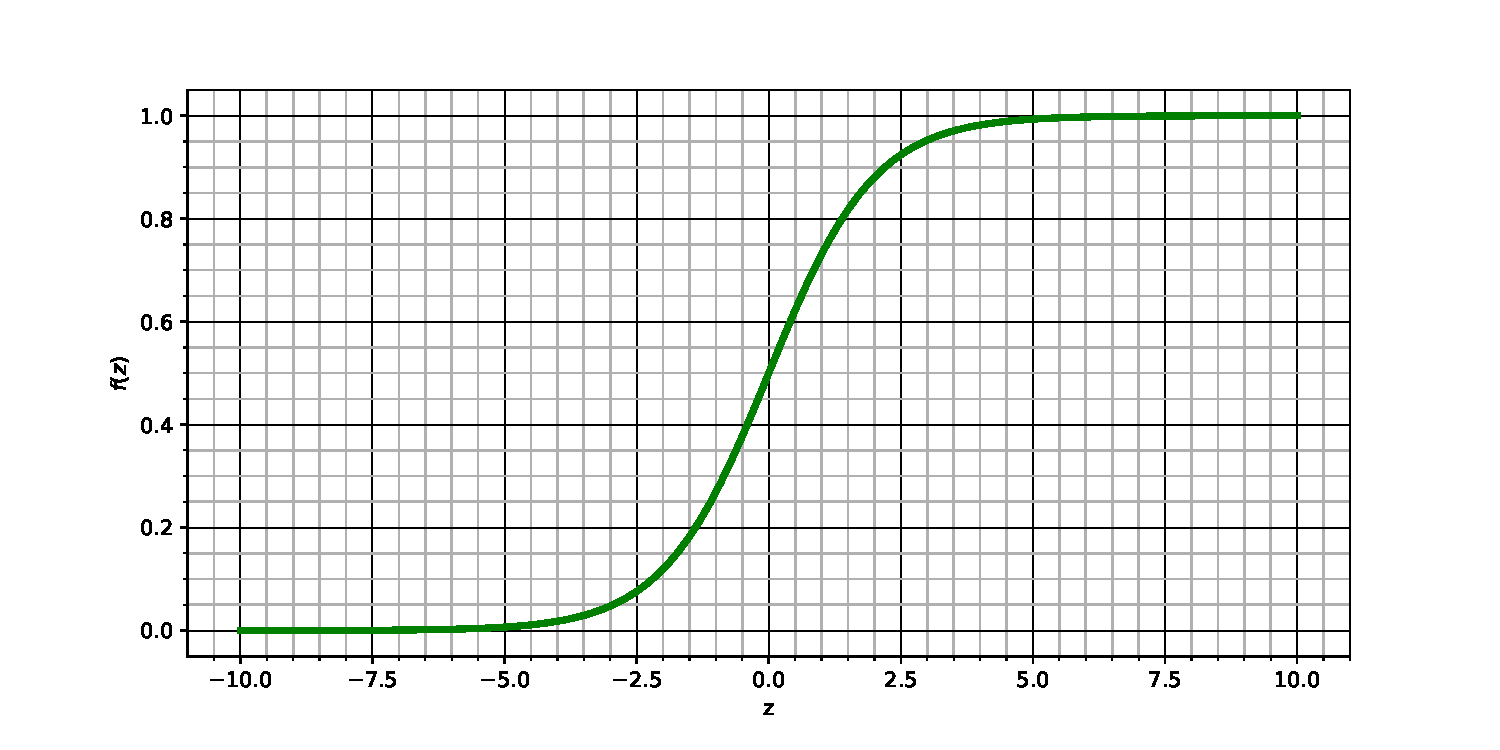
\includegraphics[width=0.99\linewidth]{images/sigmoid.pdf}
    \caption{Логистическая функция (сигмоида): $f(x)={\frac {1}{1+e^{{-x}}}}$.}
    \label{fig_7}
\end{figure}

Так как $y$ принимает только значения 0 и 1, то вероятность принять значение 0 равна:
\begin{equation*}
    {\mathbb {P}}\{y=0\mid x\}=1-f(z)=1-f(\theta ^{T}x).
\end{equation*}
Перепишем функцию распределения $y$ при заданном $x$ в следующем виде:
\begin{equation*}
    {\mathbb {P}}\{y\mid x\}=f(\theta ^{T}x)^{y}(1-f(\theta ^{T}x))^{{1-y}},\quad y\in \{0,1\}.
\end{equation*}
Это есть распределение Бернулли с параметром, равным $f(\theta ^{T}x)$.\\[5mm]
2. \textit{Случай мультиклассовой классификации (наш случай)}.\\[0.5 cm]
В отличие от бинарной классификации, где результат принимал значения 0 или 1,
т.е. $у\in\lbrace 0, 1\rbrace$, в данном случае результатом будет один из множества классов (которых
теперь больше, чем два).\\
В нашем случае $n = |y|=4,\:y\in \lbrace 0, 1, 2, 3\rbrace$.\\
В данном случае задача мультиклассовой классификации делится на 4 задачи бинарной
классификации. В каждой такой задаче бинарной классификации предсказывается вероятность
того, что $y$ относится к заданному классу.
\begin{eqnarray*}
    y\in\lbrace 0, 1, 2, 3\rbrace\\
    f^{(0)}(\theta ^{T}x)={\mathbb {P}}\{y=0\mid x;\theta\}\\
    f^{(1)}(\theta ^{T}x)={\mathbb {P}}\{y=1\mid x;\theta\}\\
    f^{(2)}(\theta ^{T}x)={\mathbb {P}}\{y=2\mid x;\theta\}\\
    f^{(3)}(\theta ^{T}x)={\mathbb {P}}\{y=3\mid x;\theta\}\\
    Prediction = \max\limits_i(f^{(i)}(\theta ^{T}x))
\end{eqnarray*}

В случае мультиклассовой классификации выбирается рассматриваемый класс, все
остальные классы при этом «объединяются» в другой класс, отличный от выбранного.
Это проделывается для каждого класса с применением для каждого случая
бинарной логистической регрессии \cite{ML_lectures}.

\subsubsection{Подбор параметров}

Чтобы подобрать параметров $\theta _{0},...,\theta _{n}$ необходимо составить обучающую
выборку (\ref{eq:eq_2}), состоящую из наборов значений признаков и
соответствующих им значений целевой переменной $y$. Формально, это множество пар
$(x^{(1)},\:y^{(1)}),\:...,(x^{(l)},\:y^{(l)})$, где $x^{(i)}\in \mathbb {R}^{n}$ --- вектор
значений признаков, а $y^{(i)}\in \{0,1, 2, 3\}$ --- соответствующее им значение
$y$. Каждая такая пара называется обучающей выборкой. Обычно используется метод
максимального правдоподобия, согласно которому выбираются параметры $\theta$,
максимизирующие значение функции правдоподобия на обучающей выборке: 
\begin{equation*}
    {\hat {\theta }}=arg\max\limits_\theta L(\theta)=arg\max_\theta \prod_{{i=1}}^{{m}}{\mathbb {P}}\{y=y^{{(i)}}\mid x=x^{{(i)}}\}.
\end{equation*}
Максимизация функции правдоподобия эквивалентна максимизации её логарифма \cite{ML_lectures}: 

\begin{eqnarray*}
    \ln L(\theta )=\sum _{i=1}^{m}\log \mathbb {P} \{y=y^{(i)}\mid x=x^{(i)}\}=\sum _{i=1}^{m}y^{(i)}\ln f(\theta ^{T}x^{(i)})+\\
    +(1-y^{(i)})\ln(1-f(\theta ^{T}x^{(i)})), \quad\text{где\:} \theta ^{T}x^{(i)}=\theta _{0}+\theta _{1}x_{1}^{(i)}+\dots +\theta _{n}x_{n}^{(i)}.
\end{eqnarray*}

Как один из вариантов для максимизации этой функции может быть применён метод градиентного спуска.
Он заключается в проведении следующих итераций, начиная с некоторого начального значения
параметров $\theta$:
\begin{equation*}
    \theta :=\theta +\alpha \nabla \ln L(\theta )=\theta +\alpha \sum _{{i=1}}^{{m}}(y^{{(i)}}-f(\theta ^{T}x^{{(i)}}))x^{{(i)}},\:\alpha >0.
\end{equation*}

\subsubsection{Преимущества}

\begin{itemize}
    \item Простота внедрения;
    \item Малый объём вычислений при классификации, высокая скорость работы,
    а затраты по памяти малы;
    \item Можно легко обновить модель для поглощения новых данных;
    \item Удобно оценивать вероятности возникновения некоторого события по значениям
    множества признаков (пригодится нам далее при вычислении p-value);
\end{itemize}

\newpage
\subsubsection{Использованная реализация}

Чтобы применить логистическую регрессию на наших наборах данных (рис. \ref{fig_6}), 
воспользуемся готовой реализацией алгоритма, которую предоставляет \textbf{scikit-learn} \cite{scikit-learn}.

Scikit-learn --- это Python-модуль для машинного обучения, построенный поверх $SciPy$
\cite{scipy} и распространяемый по лицензии $BSD$ \cite{BSD}.
В модуле Scikit-learn реализован класс $sklearn.linear\_model.LogisticRegression$, который и
предоставляет весь необходимый функционал.

\subsection{Нормировка признаков}

\vspace*{5 mm}
% Воспользовавшись реализацией логистической регрессии в модуле scikit-learn на наших обучающихся
% выборках (см. главу \ref{sec:chapter_5_1}), получим качество предсказания натренированных
% классификаторов (рис. \ref{fig_8}):

% \begin{figure}[H]
%     \centering
%     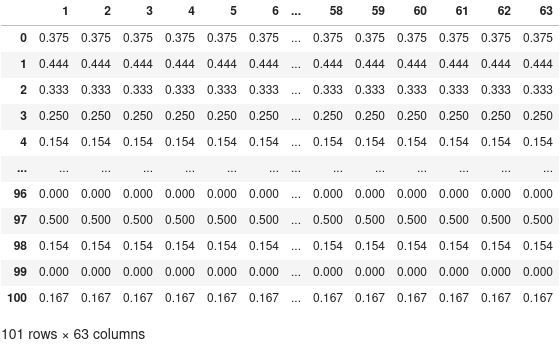
\includegraphics[]{images/8.png}
%     \caption{Результаты предсказания (score) натренированных классификаторов. По
%     горизонтали --- номер электрода, \\по вертикали --- номер участника эксперимента.}
%     \label{fig_8}
% \end{figure}

Так как значения признаков имеют малые порядки (от $10^{-14}$ до $10^{-10}$) и сильно
различаются между собой по величине, то, в виду чувствительности алгоритма
к диапазону изменений входных переменных и чтобы избежать ухудшения результатов обучения,
перед использованием логистической регрессии необходимо провести
\textit{нормировку признаков.}

%\subsubsection{Описание}

В машинном обучении нормировкой признаков называют метод предобработки числовых признаков
в обучающей выборке, чтобы привести их к определённой общей шкале (в нашем случае
к отрезку [0, 1]) без потери информации о различии диапазонов \cite{ML_lectures}.

Необходимость нормализации вызвана тем, что разные признаки обучающей выборки
могут быть разных масштабов и изменяться в разных диапазонах.

В этом случае возникает нарушение баланса между влиянием входных переменных,
представленных в разных масштабах, на выходную переменную. Т.е. это влияние обусловлено
не реальной зависимостью, а изменением масштаба. В результате, обучаемая модель
выявит некорректные зависимости.

В модуле содержится несколько реализаций нормировок признаков, иллюстрации которых приведены ниже:

\begin{figure}[H]
    \centering
    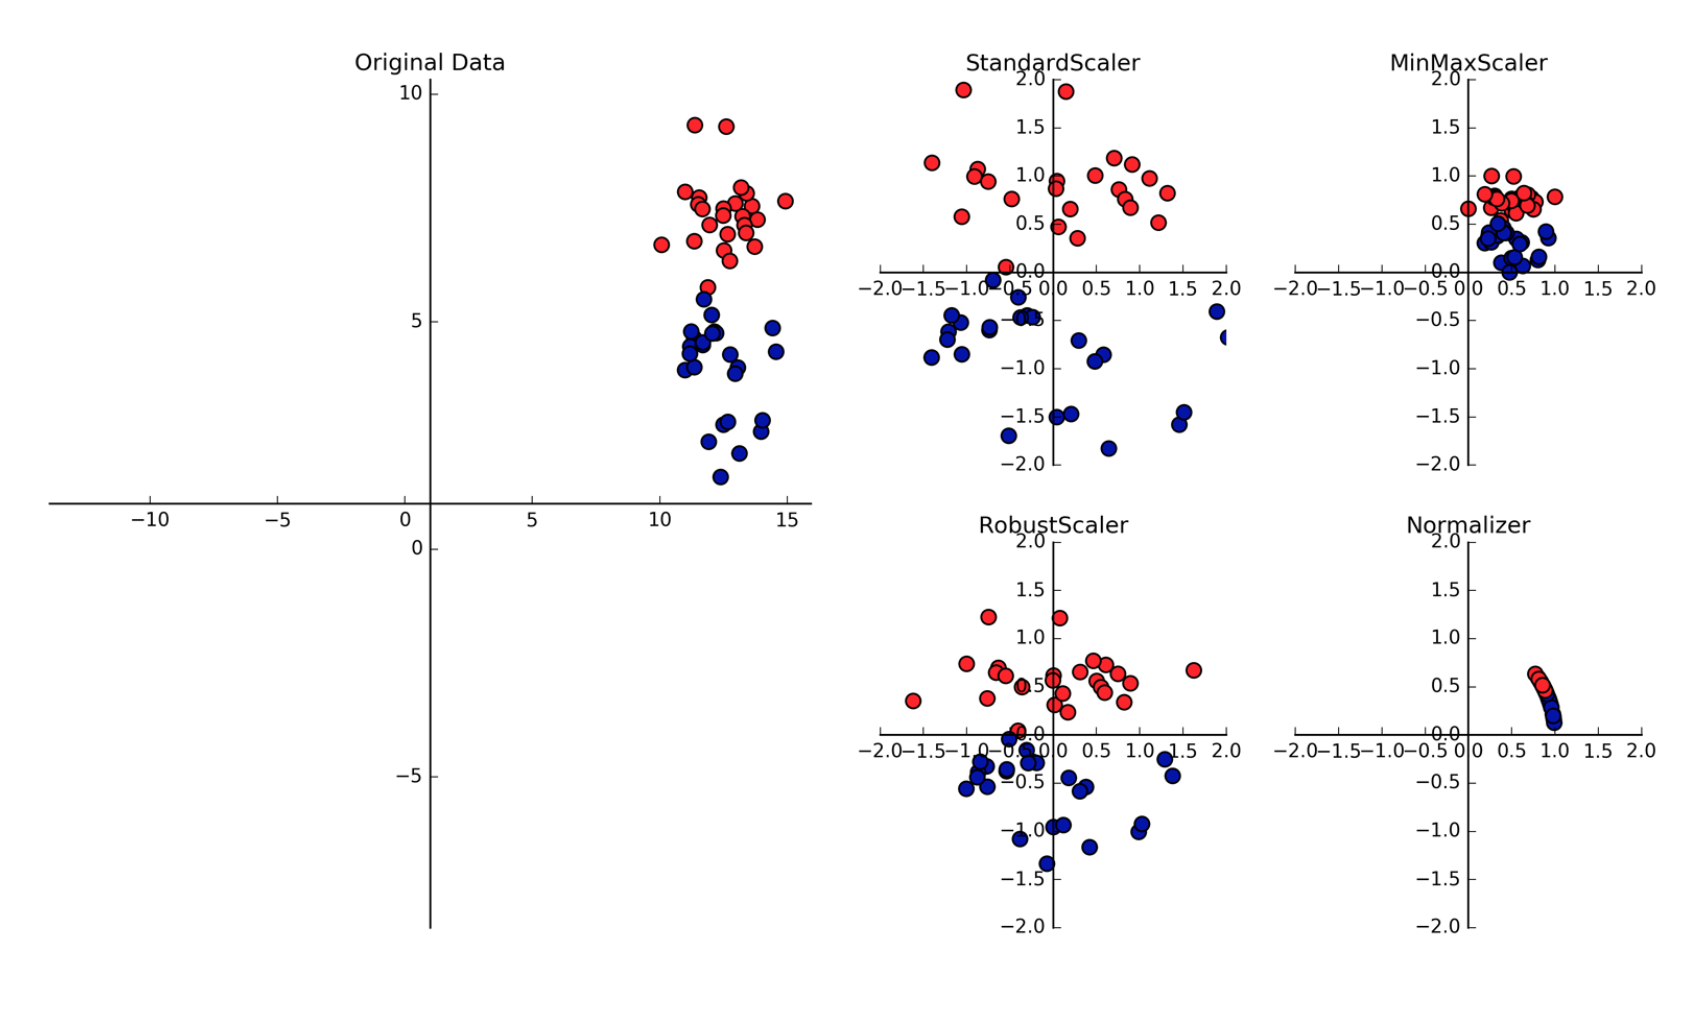
\includegraphics[width=\linewidth]{images/scaling.png}
    \caption{Иллюстрация нормировки признаков в зависимости от различных реализаций
    (MinMaxScaler, StandardScaler, RobustScaler, Normalizer),
    содержащихся в модуле scikit-learn \cite{scikit-learn}}
    \label{fig_scaling}
\end{figure}

\subsubsection{Минимаксная реализация}

Существует несколько реализаций методов нормировки признаков в модуле scikit-learn.
В данной работе была использована минимаксная реализация \cite{scikit-learn}.

\begin{figure}[H]
    \centering
    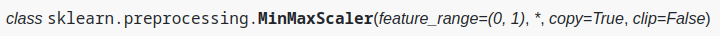
\includegraphics[width=\linewidth]{images/9.png}
    \caption{Минимаксная реализация модуля scikit-learn}
    \label{fig_9}
\end{figure}

Данная минимаксная нормировка реализуется по формуле:
\begin{equation*}
    \hat{x}=\frac{x-\min(x)}{\max(x)-{\min(x)}},
\end{equation*}
где $x$ является исходным значение признака, а $\hat{x}$ -- преобразованное к заданному диапазону (к отрезку
$[0, 1]$) значение.

\subsubsection{Применение}

Итак, воспользуемся готовой реализацией и проведём нормировку признаков.

\begin{figure}[H]
    \centering
    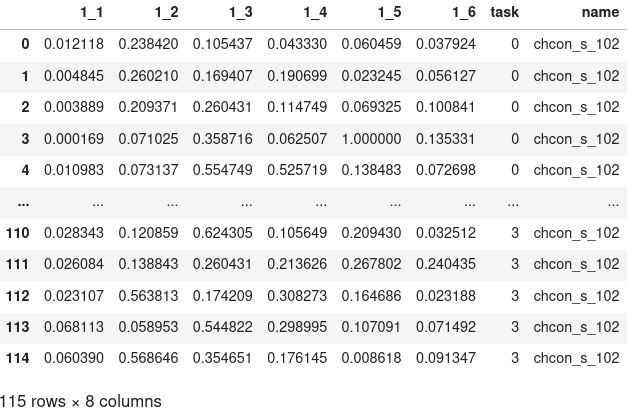
\includegraphics[width=\linewidth]{images/10.png}
    \caption{Пример одного из наборов данных после нормировки признаков. (можно сравнить
    с рисунком \ref{fig_6})}
    \label{fig_10}
\end{figure}

\subsection{Применение логистической регрессии}

На обучающихся выборках типа (\ref{eq:eq_2}) используем логистическую регрессию, чтобы
узнать как амплитуда биоэлектрической активности, регистрируемой электродом с конкретной
зоны мозга, в отдельности влияет на результат классификации типа решаемой задачи и выявить
какие из них больше всего влияют на результат.

\subsection{Метрика оценки качества}

Для оценки качества построенных линейных моделей используем метрику
\textit{accuracy score}.

Перед тем, как перейти к описанию самой метрике, введём матрицу ошибок (сonfusion matrix) для описания метрики
в терминах ошибок классификации.
Пусть у нас есть два класса и алгоритм, предсказывающий принадлежность каждого
объекта к одному из классов, тогда матрица ошибок классификации будет выглядеть следующим
образом:

\begin{figure}[H]
    \centering
    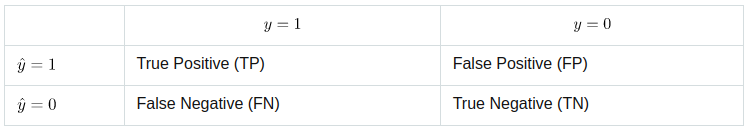
\includegraphics[width=\linewidth]{images/11.png}
    \caption{Матрица ошибок классификации}
    \label{fig_11}
\end{figure}

% \begin{table}[H]
%     \begin{center}
%         \caption{Матрица ошибок классификация}
%         \begin{tabular}{ | c | c | c |}
%             \hline
%              & $y=1$ & $y=0$ \\ \hline
%             $\hat{y}=1$ & True Positive (TP) & False Positive (FP)\\
%             \hline
%             $\hat{y}=0$ & False Negative (FN) & True Negative (TN)\\
%             \hline
%         \end{tabular}
%         \label{fig_11}
%     \end{center}
% \end{table}

Здесь $\hat y$ — это ответ алгоритма на рассматриваемом объекте, а $y$ — истинная метка класса на
этом объекте. Ошибки классификации бывают двух видов: False Negative
(FN) или ошибка 1-го рода и False Positive (FP) или ошибка 2-го рода \cite{ML_lectures}.\\
\textit{Accuracy score} --- метрика, показывающая долю верных ответов алгоритма:
\begin{equation*}
    \large accuracy\: score = \frac{TN+TP}{FP + FN + TP + TN}
\end{equation*}



%\subsection{Проверка гипотезы} % возможно вынести это в отдельную главу и назвать "проверка на достоверность" полученных результатов